\documentclass[10pt,twocolumn]{article}
\usepackage{graphicx}
\usepackage{changebar}

\begin{document}

\title {Why robot programming is hard}
\author {Tessa Lau \\
Savioke Inc.\\
Santa Clara, CA\\
{\tt tlau@savioke.com}
}
\maketitle

% Hai Nguyen's ROCON
% Maya's Robot PBD
% Strips style robot planning


I never thought I would be a roboticist. In grad school, our robotics team spent months teaching little robot dogs to play soccer and solving other seemingly simple problems. Far better to work in the world of software, I figured, where the systems I built could make a real difference in people's lives. Software could automate repetitive tasks in computer use and free people from mundane work. So instead I developed expertise in human-computer interaction and intelligent user interfaces. My chosen field, end user programming, has the potential to enable millions of ordinary computer users to customize and adapt systems to their own needs.

But the world is changing. Computing has moved off the desktop and into the smartphones, smart environments, and the world around us. Innovation is happening in the physical world, using computing to effect material change in our environment. The past decades have seen industrial robots increase manufacturing efficiency on the factory floor. Even more, we are now seeing robots tackle tasks from our daily lives. Robotic vacuum cleaners are changing the way we clean our homes. Robotic lawnmowers keep the yard tidy without having to lift a finger. Nest's robotic thermostat learns your habits and keeps your home at the optimal temperature. Google's driverless car could change the way we commute.

All these innovations have become possible through multiple advances: in sensor technology, which robots use to perceive the world around them~\cite{henry-iser10}; in planning and navigation, which enable robots to move around in the world unaided~\cite{jackel-cacm07}; in human-safe motion controllers, which let robots move their limbs without endangering the people around them~\cite{kemp-ieee07}; in the ROS open source robot operating system, which enables roboticists to build on each others' work without starting from scratch~\cite{quigley-icra09}; and many more advances in the broader field of robotics.

Yet the holy grail of personal service robots remains elusive. I believe there are three main reasons. First, there is a wide variety of tasks that people want service robots to perform, ranging from folding laundry, to finding lost car keys, to picking up the kids' toys, or doing the dishes and putting them away. Second, these tasks must be performed in a variety of environments, including cluttered homes and kitchens with different affordances such as modern drawer pulls or faucet handles. Finally and most importantly, the robots themselves must be easy to operate by non-technical people.

We have started to see robots enter the marketplace that address two out of those three challenges. For example, iRobot's Roomba\footnote{http://www.irobot.com} only vacuums floors, but it does so in a variety of environments and is simple to use even by non-technical folks. On the other hand, Rethink Robotics' Baxter robot\footnote{http://www.rethinkrobotics.com/products/baxter/} can be easily programmed to perform a variety of tasks in light industrial settings, but its lack of mobility makes it less suitable for the home. As another example, Willow Garage's PR-2 robot has been programmed to perform a variety of household tasks, in a variety of environments, but can only be operated by highly skilled roboticists.

Yet I believe the time is ripe for a breakthrough in personal service robotics, starting with robots that perform simpler tasks in relatively structured environments such as hospitals or hotels, and driven by better design and usable interfaces that enable them to be used by non-expert users.

\section{Case study: Robots for Humanity}

One important use case for personal service robots will be in-home care and assistance for disabled adults. The Robots for Humanity project~\cite{rfh}, a collaboration between Willow Garage and Georgia Tech, aimed to develop technology that enabled persons with motor impairments to perform personal care tasks that they otherwise might not have been able to perform without assistance, such as picking up a dropped object, fetching a towel, or even scratching an itch. Its first prototypes enabled Henry Evans, a mute quadriplegic, to act in the world for the first time since a brainstem stroke left him paralyzed. Through physical therapy, Henry had regained the ability to make limited head motions (enough to control a cursor with his gaze) and to click a button with one finger.  Using an interface custom designed for him, Henry was able to instruct Willow Garage's PR-2 robots to open cabinets in his home, fetch food from the refrigerator, and even dole out candy to trick-or-treating kids on his behalf.

Yet our experience with Robots for Humanity underscored how difficult it was for ordinary mortals to instruct robots what to do. Even using state-of-the-art robot visualization software developed at Willow Garage, simple teleoperation tasks such as opening a cabinet door was very difficult for Henry to accomplish. While Henry had only limited interaction capabilities, he was also strongly motivated because he has no alternatives. Able-bodied consumers, on the other hand, would quickly lose patience and simply fetch the towel themselves. If the state of the art in robot operation is so time-consuming, what hope do we have that ordinary mortals will be able to operate robots to perform these tasks in their own homes?

Granted, designing teleoperation interfaces for motor-impaired users is deliberately trying to solve the hardest problem first.  Yet while Henry's case highlights the challenges of creating usable assistive robotics interfaces, it also illustrates the enormous benefit to humanity of enabling disabled adults to regain some of their independence.

With this goal in mind, personal service robots are more than a consumer toy, but a technology that could changes people's lives for the better.  Why, then, are robots still so difficult to use? What makes robots so difficult to operate?

\section{Robot programming}

Wikipedia defines computer programming as follows (italicized text added for clarification):

\begin{quote}
The purpose of programming is to find a sequence of instructions that will {\it [cause the computer to]} automate performing a specific task or solve a given problem.
\end{quote}

If you replace computer with robot, we come to a definition of robot programming: finding the right series of instructions that cause a robot to automate a task or exhibit a certain behavior. Every robot makes available a certain set of functionality -- its user-visible API. These are the primitive behaviors that have been programmed into the robot and can be activated by its user. End users must select which behavior to call when, in order to make the robot do what they want.
%Anyone who operates a robot, including consumers who purchase one for their home, will be programming the robot according to this definition.

Many of the lessons learned from the fields of end user programming~\cite{dontcheva-nocode} and end user software engineering~\cite{ko-acm11} also apply to robot programming, though robots' physical embodiment leads to additional challenges. Based on my experience in both end user programming and robotics, I believe that the difficulty of the robot programming task boils down to several factors:

\begin{itemize}
\item {\bf Direct contact with the robot/task}: programming is easier if the user can see and touch the robot and its desired task. Control from a distance makes the programming process harder~\cite{chen-ieeetos07}. For example, robots that are sent into natural disaster zones as first responders may have to be operated from a distance, which increases the programming task's difficulty because the operator's senses are limited to what can be perceived through the robot's own cameras or sensors.

\item {\bf Task/environment variance}: if the task to be performed is always the same, the programming task is easier than if the goal task changes significantly or if the environment in which the robot must operate is changing. The program must be generalized to handle this variance, which makes the programming process more difficult.
% REF: something from the EUP literature? Andy Ko or Margaret Burnett?

\item {\bf Goal specification}: some tasks are easy to describe, such as navigation goals specified by a single point in 3-dimensional space. Other goals, such as washing the dishes or tidying up, are more difficult to specify. Successful completion may be more dependent on how exactly the robot performs the task. Generally speaking, the more difficult it is to frame the goal specification, the more difficult the programming task will be~\cite{ko-vlhcc04}.

\item {\bf Amount of autonomy}: robots are gaining the ability to perform some functions autonomously, such as spatial navigation and object manipulation.  The less autonomy exhibited by the robot, the easier it is to program the robot, because increased autonomy requires the programmer to develop more complex mental models of the robot's perceptions and behavior~\cite{kulesza-chi12}. Teleoperation interfaces are fairly easy to use because there is generally a one-to-one mapping between the user's inputs and the robot's behavior. Once a robot starts to act autonomously, understanding its behavior (and debugging it!) becomes more challenging.
\end{itemize}

For personal robotics to truly succeed, regular people will need to use robot programming interfaces to tell robots what to do. These interfaces for robot programming will need to be simple enough for ordinary consumers to be able to pick up and use. Until users are able to instruct robots quickly and with low effort, personal robotics will be limited to niche markets. Why is end user robot programming so challenging? Several compounding factors make it more difficult than normal computer use.

The story begins with a look at the state of the art in robot software today.


\section{The state of the art}

% History of ROS
% Invented by Willow Garage, new operating system for diverse robots
% Current reach
% Running on robots from PR2 to android-powered XXX
% Provides very rich control substrate for programming the behavior of complex robots

The Robot Operating System\cite{ros} is one of the software advances that supports the rapid development of new robotics technology.  First developed in 2007 at the Stanford Artificial Intelligence Laboratory, ROS was maintained by Willow Garage from 2008-2013 and has since transitioned into the stewardship of the non-profit Open Source Robotics Foundation\footnote{http://www.osrfoundation.org/}.

ROS provides a distributed publish/subscribe messaging platform for a collection of {\em nodes} to communicate with each other. Each node encapsulates a small amount of robot functionality, and interfaces with the rest of the ROS ecosystem to make that functionality available through a common interface. For example, ROS nodes exist to stream sensor data from webcams and laser rangefinders, control the motors in robot arms, plan a path from one point to another, and recognize graspable objects in an image.

Before ROS, roboticists had to create the software to control their robots from scratch, each doing the same work to create device drivers and rebuild libraries for their specific robot's hardware.  Now, ROS has been ported to around 100 different models of robots worldwide\footnote{http://www.ros.org/wiki/Robots}, enabling roboticists to quickly bring a new robot model online.

\begin{figure*}[tbh]
\center\scalebox{0.13}{
	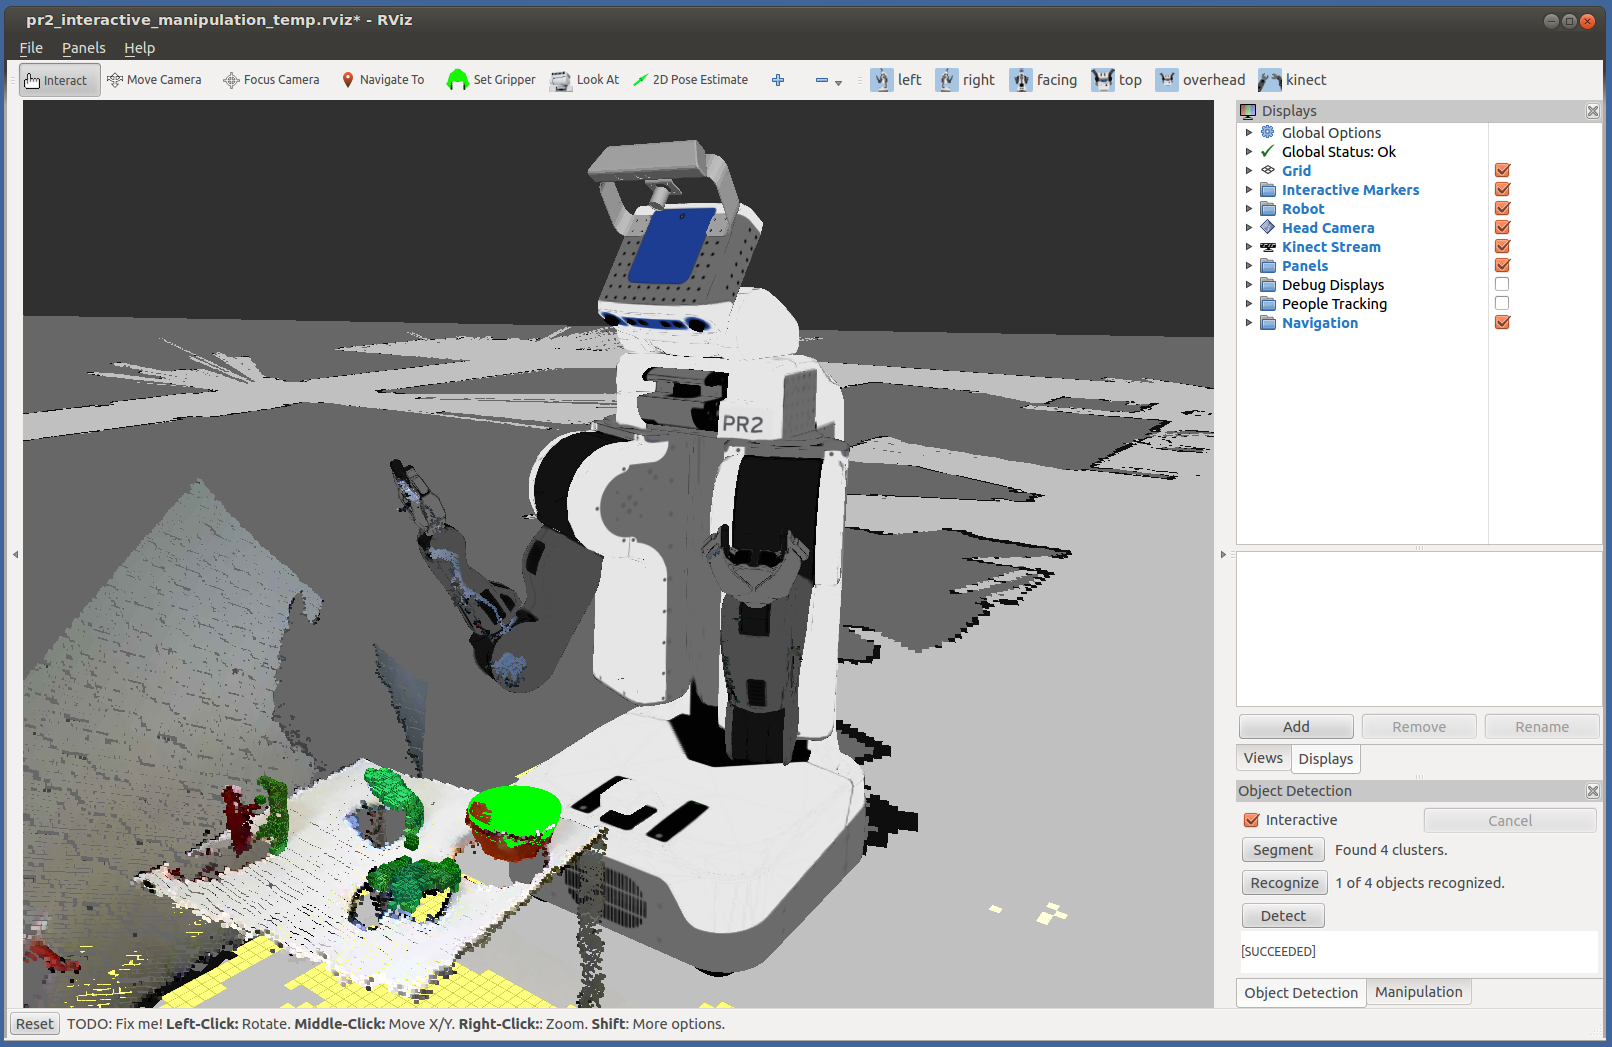
\includegraphics{rviz1.png}
	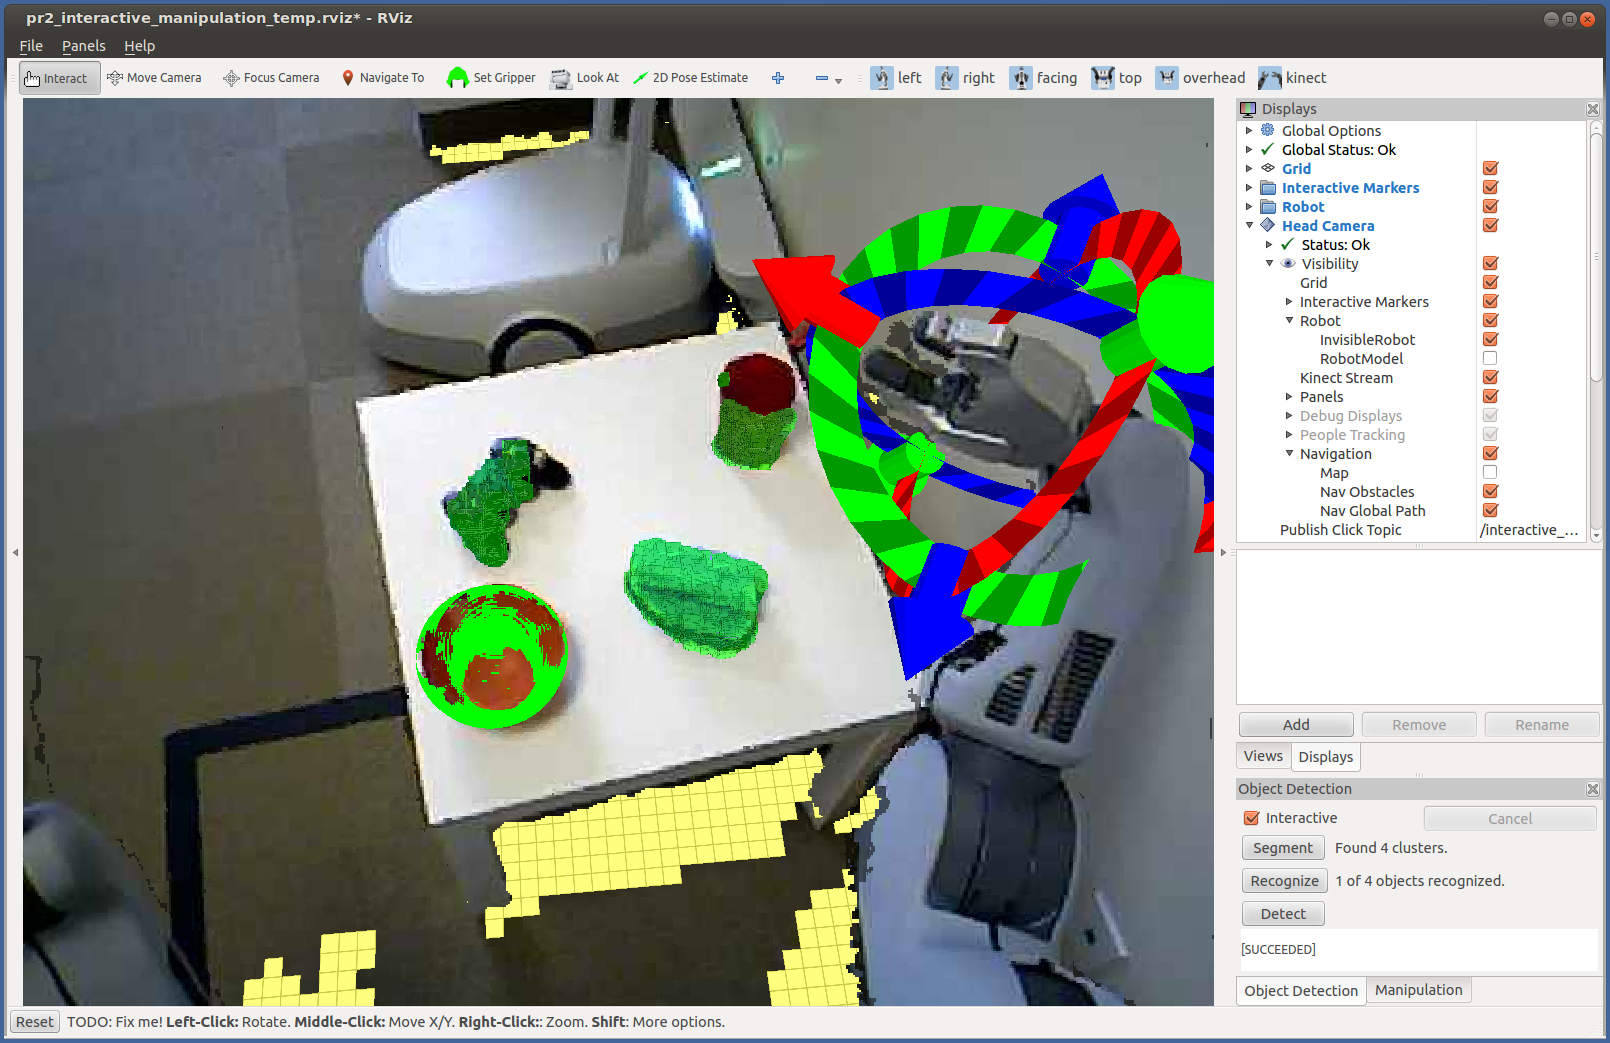
\includegraphics{rviz2.png}
}
\caption{RViz interfaces for robot visualization and control}
\label{rviz}
\end{figure*}

However, ROS provides a fairly low-level interface to robot control. Designed for roboticists, the RViz interface (Figure~\ref{rviz}) displays all the sensor feeds coming from the robot and lets one send low-level motion commands to the robot such as rolling forward or rotating its shoulder joint. The figure shows two different perspectives on the same robot examining objects on a table in front of it. The left figure shows a third-person view of the robot and the table, rendered on top of a two-dimensional map of its environment (the gray pattern in the background). The green overlays on top of the tabletop objects indicate that they are recognized by the system as objects that can be picked up. The yellow grid pattern indicates horizontal surfaces that are detected, such as the floor.  The right figure shows the view as soon from the robot's head-mounted camera. The red/green/blue arrows are control markers that can be used to rotate and move the robot's gripper in all directions~\cite{gossow-ieee11}.

\section{Why robot programming is hard}

The Rviz interface, while well suited for roboticists who need to examine the low-level sensor data and messages being processed by the robot, is not very user-friendly. It also illustrates some of the difficulties inherent in robot programming.

\subsection{Concurrency}

% ROS nodes
% multiple parts of robots (head, arms, base)
% callbacks, coroutines, threads

Many activities of daily living require coordinated action amongst multiple limbs. Anyone who has broken an arm, for example, understands the difficulty of trying to unscrew jar lids, pick up bulky objects, or chop vegetables with only a single arm. Controlling both arms simultaneously to perform coordinated actions is a matter of concurrent programming.

The problem becomes even more complex with robots that have many moving parts.  For example, Willow Garage's PR-2 has two independently controlled 7-DOF arms, a head that can pan and tilt, a torso that can be raised and lowered, and a base that can move and turn in all directions. Robots are also equipped with a slew of sensors including cameras, depth sensors, laser rangefinders, touch sensors, and feedback about its electrical and motor systems. These sensors and actuators must be operated together in coordination to produce a desired robotic behavior.

Concurrent programming is notoriously difficult even for professional programmers due to the possibility for race conditions and the complexity of reasoning about what the program does~\cite{shavit-cacm11}. Professional programmers learn to use advanced techniques such as multi-threading, event-driven callbacks, and coroutines in order to specify concurrent behavior in programs. Yet these concepts are notoriously difficult to use and debug, even for trained programmers; how can we expect non-technical users to be able to do the same, in order to instruct multi-limbed robots?

In addition to the low level concurrency needed to control multiple robot parts, there is also a need to specify concurrent robot behavior at a higher level~\cite{cakmak-hri13}. For example, a user may want to give the robot background tasks (such as cleaning or plugging oneself in when the battery is low) which might be scheduled in concert with foreground tasks (such as fetching a drink).

%Most robot programs can be simplified by only controlling one moving part at a time: first move the base, then raise the torso, then position the left arm, then position the right arm, finally open the cabinet. For many tasks this is a reasonable solution. However there is a subset of human tasks for which we need multiple parts moving simultaneously, such as picking up a heavy or bulky object with two hands, or turning one's head to look where one is going.

End user programming systems have tried various techniques to deal with the problem of concurrency. Some systems visualize the different components on a timeline. This approach is popular with media creation tools such as Apple's GarageBand\footnote{https://www.apple.com/mac/garageband/} or Autodesk's 3D Studio Max\footnote{http://www.autodesk.com/products/3ds-max/overview}. A second paradigm, taken by visual programming languages such as Scratch~\cite{scratch}, makes the notion of time a global constant and runs all blocks of user code simultaneously in the virtual environment. More research is needed to discover what paradigm works best for controlling robot parts concurrently.

% A second option for concurrency is to reduce the end user's need to write concurrent programs by defining new primitives that cover the common cases where concurrency is needed.  For example, a robot navigation algorithm may include the ability to turn the robot's head to look in the direction of motion, eliminating the need for the user to specify this complex behavior.  As another example, a two-armed robot could have both arms linked in a mirror configuration so that a command to move one arm would cause the other to mirror its motion, thus enabling the robot to pick up symmetric objects with two hands.

\subsection{Uncertainty}

% World changes out from under you
% Hardware fails
% Incomplete world models
% Bayesian methods, probabilities

Another challenge that robot programmers face is specifying how a robot should behave in an uncertain world. The world is constantly changing: any model that a robot could build of where things are located will be obsolete by the time it turns around~\cite{fox-jair99}. People walk around, objects get lost, furniture gets moved. Moreover, limitations in current sensing technology make it difficult to build a perfectly accurate model of the world~\cite{kemp-ieee07}. For example, differences in lighting make the same object look very different to an RGB camera. Therefore a robot cannot necessarily trust what it perceives, and it must be able to deal with the possibility that what it thinks is true is not actually true.

In addition, robot hardware itself often produces unpredictable results. Unlike software, mechanical parts can slip, burn out, or break. They take time to actuate and do not come to a stop immediately. Giving a robot the same instruction multiple times may or may not result in the same outcome each time.

Thus robot programs must have mechanisms in place to deal with uncertain truth and unpredictable hardware. Robot control loops usually sense the physical hardware during operation to determine whether a motion was carried out successfully.
If an operator is not physically co-located or co-temporaneous with the robot, she cannot see whether the robot carried out the desired motion, so she must think through possible outcomes while writing a program and craft appropriate responses for each eventuality. For example, while instructing a robot to pick up an object, a programmer must specify what to do if the object is not {\em where} it thinks it is, is not {\em what} it thinks it is, or if the robot fails to perform the desired grasp. Should it simply try again? Move a little bit to get a better view and then try again? Ask a human?

In order to deal with these various types of uncertainty, professional programmers learn to use probabilistic models~\cite{darwiche-cacm10} and craft fault-tolerant code~\cite{wright-cacm09} with frequent error checking. Nguyen's ROS Commander (ROSCo) system is an end-user programming system aimed to enable home users to define new behaviors for PR2 robots by visually crafting finite state machines~\cite{nguyen-icra13}. ROSCo XXX TODO

which seems like too much to ask of casual programmers who just want to teach their robot to do something useful in the home.


\subsection{Commonsense reasoning}

Reasoning about objects in the world requires some amount of common sense which has yet to be programmed consistently into robots. For example, a robot who has been asked to pick up and deliver a coffee cup may well select a grasp that involves dipping its fingers into the liquid and picking up the cup by its side wall. Although the grasp would be valid, this behavior would be judged somewhat undesireable by human observers.

As another example, robots that are capable of automated navigation may fail to observe human norms when navigating through human spaces. The custom of staying to the right when passing in a hallway, for example, can cause confusion if a robot charges down the middle of the hall and does not yield to oncoming passerby.

Endowing computers with common sense is still an active research area~\cite{mueller-cacm09}. Techniques for making use of common sense reasoning have not yet made it into the vocabulary of professional programmers. Yet these concepts will be taken for granted by end users of robots, who will expect their robots to obey common social norms as they perform their tasks.

\subsection{A 3D world}

% Robot arms have 7DOF
% grasps require 6D
% world is 3D
% quaternions, matrix manipulation
% specialized I/O devices

Unlike traditional computer interfaces which are limited to two dimensions, robot control requires manipulating objects in a three-dimensional world. Visualizing a 3D world on existing 2D displays requires the extra dimension to be projected down into two dimensions, giving rise to the popular ``first person shooter'' style of interface. These interfaces display the world as perceived from a virtual camera, where objects can be occluded by other objects. Additional camera controls are needed to pan/zoom around the space to overcome occlusion. These controls are often non-intuitive, even to seasoned computer users.

Occlusion presents a challenge because robots must perceive an object in order to manipulate it.  Often times, the robot itself might occlude the object it is trying to manipulate! For example, consider a humanoid robot with head-mounted vision sensors using an arm to pick up an object from the table in front of it. While moving the arm into position to grasp the object, the arm will likely come between the head and the object, obscuring the robot's vision.

One solution has been to mount additional cameras on different parts of the robot, such as on the robot's forearm or wrist, to get a better view on the object being picked up. However, making sense of multiple translated and rotated video streams can be confusing for those of us accustomed to perceiving the world only through head-mounted eye sensors!

Typical input devices such as mice and touchscreens are also only good for interacting in two dimensions. For example, tapping on a point in a camera image does not uniquely identify a point in 3D space, but a line of possible points. When telling a robot to put something down, how can it know which of those points was meant? Current interfaces, such as the RViz display shown in Figure~\ref{rviz}, require complex camera manipulation and precise 3D positioning in order to uniquely specify the desired location.

%\section{7-DOF arms}
%
%A different aspect of high-dimensionality comes from the design of robot arms. A solid object in 3D space has six degrees of freedom (DOF): three dimensions to specify its position, and three more to specify its rotation. If a robot arm had only 6-DOF and was trying to execute a specific grasp of a particular object, such as picking up soda can from the side, there would be only a single arm configuration that would allow the gripper (a robotic hand) to pick up the can. In contrast, human arms and advanced robot arms have 7-DOF, which allows them one extra dimension of flexibility in achieving those grasps. To visualize this, imagine grasping a soda can on the table in front of you and then flapping your elbow up and down while keeping the can stationary. That extra degree of freedom enables your arm to take on all those different shapes while still achieving the desired grasp.
%
%Interfaces for robot arm teleoperation typically involve setting the position or angle of each joint in the arm individually. For example, a tablet-style interface might have fourteen buttons, one pair used to increase or decrease the angle of each joint in the arm. That additional degree of freedom makes it easier to identify a valid arm configuration for executing a grasp, since only one of many valid configurations must be found, not the unique one.  However controlling each individual joint position by clicking on buttons is tedious. Additionally, since the allowable joint positions are not completely independent, finding a correct solution is often done through trial and error.
%
%Toolkits for doing automatic motion planning are maturing, which will simplify the problem of robot arm control from how the arm should move in fine-grained detail to specifying only the high-level target position and orientation. Yet the challenge of specifying that 6-DOF target position and orientation still remains, and this will continue to be a challenge for easy-to-use robot interfaces that work with existing 2D displays and input devices.
%

%There is a tradeoff between exposing these joint limitations to the programmer, which allows precise yet complex control, versus insulating a programmer from those considerations, which may lead to unpredictable behavior that is difficult to debug.

% Yet positioning an arm through direct manipulation or teleop is relatively easy compared to doing it programmatically. In order to program an arm, one must first specify {\em where} it should go.  Expert roboticists represent the world in terms of {\em reference frames} (coordinate systems that are defined relative to a fixed position). For example, one reference frame could be relative to the building, with the front door being at coordinate (0, 0).  Other reference frames are defined relative to stationary parts of the robot, such as its base (if it is on wheels), the head-mounted camera, or the right elbow joint.
% 
% Sending an arm to a specific position is useful for robot tasks such as, for example, looking at what it is holding by moving its hand to half a meter in front of its face. This half-meter is most reliably specified in the reference frame relative to the robot's head. Given this goal position, the programmer must find a series of arm configurations that moves the arm to the desired place, while avoiding contact with obstacles in the environment.

% such as the base or the head-mounted camera) and use matrix algebra to convert between different frames of reference. Robot joint positions are typically specified relative to their own reference frame; for example, a robot's wrist, which is located at the end of its arm, can be commanded to rotate around the axis that is aligned with the robot's forearm (similar to the motion we use to screw in a light bulb). Calculating the absolute position of a robot's hand (for example, to determine whether it is near the door handle) requires a series of complex matrix calculations starting from the position of its base, through its shoulder, and all the joints, down to the hand. The opposite problem, calculating the joint positions required to get the hand to a particular position, is called {\em inverse kinematics} and is typically solved using either analytical equations or heuristic approximation methods.


\section{End user programming for robots}

The field of end user programming~\cite{lieberman-yourwish,dontcheva-nocode} has developed a variety of solutions to enable users of software systems to create or modify software artifacts without having to learn the intricacies of programming.  

The key insight for these EUP systems is to reduce the complexity of a programming task through simplification. The three primary methods include (a) visual programming: simplifying or eliminating tricky syntax through graphical representations; (b) domain-specific languages: limiting concepts to only those necessary in a particular domain of use, such as spreadsheet formulas; and (c) programming by demonstration or example: letting users focus on concrete examples rather than difficult abstractions.

However, this simplicity typically comes at the price of expressiveness. By reducing the complexity exposed in an interface, we also reduce the number or variety of functions that can be performed in that interface. In order to make robots that are more tractable for non-technical users, we will have to simplify key aspects of robot behavior, thus sacrificing robots' ability to perform a full range of behavior.

%The current generation of commercial home robots illustrates one extreme end of the simplicity versus expressiveness tradeoff. iRobot's successful Roomba line of vacuum-cleaning robots\footnote{http://www.irobot.com/us/learn/home/roomba.aspx} sports a single-button interface that simply says ``Clean''. While the robot will eventually clean your floors, you lose control over how exactly it does so, as it performs what seems like a random walk through your home.

%The next generation of commercial robots in this space will likely look like Rethink Robots' Baxter system\footnote{http://www.rethinkrobotics.com/index.php/products/baxter/}.  Baxter is a two-armed manipulator than can be programmed by demonstration to automate factory work simply by guiding its arms to the appropriate position and tapping icons on the robot's ``face''.  Unlike past demonstration-based robots which mindlessly repeated the same motions, Baxter has an intelligent motion planner which can immediately cease moving the arms if it detects something in the way, such as a human walking into its workspace.

%This style of programming makes it possible for people to specify the robot's behavior directly on the robot, without having to deal with any abstractions. In addition, Baxter performs its work in a human-safe way, immediately ceasing motion if it detects that a human has moved into its path, enabling it to work side by side with factory workers unlike previous generations of industrial robots.

%Roboticists are hard at work developing increasingly autonomous robot capabilities for well-specified tasks such as 2D navigation (getting from point A to point B within a building), arm motion planning (moving the gripper to a specified position and orientation while avoiding obstacles)\footnote{MoveIt!, http://moveit.ros.org}, and recognizing and picking up discrete objects on a flat surface. Autonomy is key for enabling robots to automatically perform longer and more complex tasks on their own.

\subsection{Higher-level primitives}

One way to trade off expressiveness for simplicity is to abstract away details of robot behavior into higher-level primitives. This abstraction can be difficult for roboticists to accept, who have become accustomed to having fine-grained control over robot behavior and error handling. Yet abstracting away these details is going to be critical for end users to be able to develop a working understanding of a robot's functionality.

%Our approach to designing end-user-programmable interfaces is to craft these autonomous components into a good set of {\em primitives} in an end user programming language, such that a non-expert would not have to ``look inside the box'' to understand how each one works.

Roboticists can then implement these primitives using advanced techniques to solve the difficult problems encountered during robot programming.
For example, a good autonomous navigation component could incorporate a set of recovery behaviors to try on navigation failure, such as turning around, waiting for people/obstacles to clear out of its path, and backing up and retrying. It could also bake in some concurrent strategies, such as turning the head to look in the direction the robot is going. 

%Encapsulating all this functionality into a single component with a well-defined interface makes it easier for end user robot programmers by giving them more reliable, easier to understand components they can assemble into programs.

\begin{figure*}[tbh]
\center\scalebox{0.40}{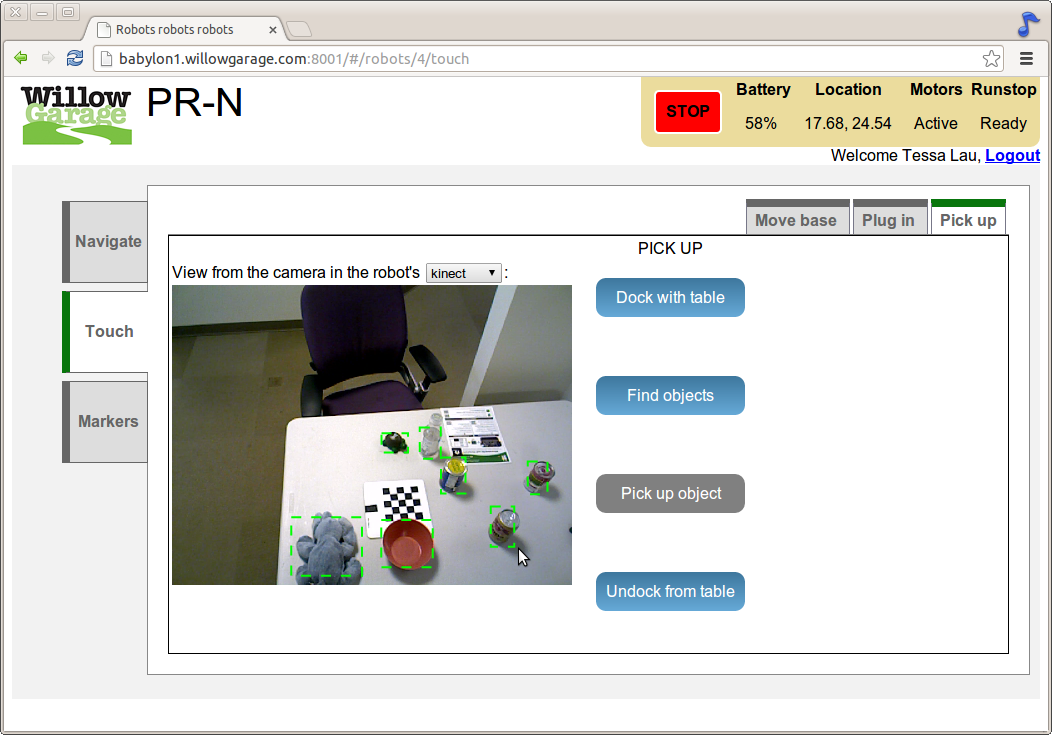
\includegraphics{contops.png}}
\caption{Continuous Ops interface for picking up objects on a table}
\label{contops}
\end{figure*}

We made use of these autonomous functions to develop a system at Willow Garage called Continuous Ops (short for ``Continuous Operations'') that enabled casual users to control PR-2 robots through a web interface (Figure~\ref{contops}).
The interface was inspired by the head of Willow Garage, who noted that even though he had a lab full of robots, he himself wasn't able to show off any of the functionality of his robots to visitors without a roboticist present to operate them.

In response, we developed a web interface, accessible from standard laptops or tablets, that provided the ability to tell a PR-2 robot to perform a variety of tasks.  It could unplug itself from the power supply, navigate autonomously to anywhere in the buliding, position itself in front of a table, automatically identify graspable objects on that table, and pick up an object.
The interface enabled non-technical users to activate several core autonomous functions of the PR-2 through an easy-to-use interface.

The drawback of this interface was that the user lost fine-grained control over exactly how the robot performed these tasks. For example, the interface only supported using the robot's right arm to pick up an object; the left arm was unused. It did not allow the user to specify exactly how to pick up an object (e.g. from above or from the side), even though these parameters can be customized at a lower level of control. 

The challenge in designing a simpler interface is to carefully craft exactly which functionality to expose, and which functionality can be safely hidden from casual users.  For the intended users of the Continuous Ops interface, the provided functionality was sufficient and satisfied the requirements of being easy to use and always available. In fact, we heard of several cases where people used the interface remotely (e.g. while away at a conference) to show off the functionality of the robots in the lab.

\subsection{Shared autonomy}

Another way to simplify the programming problem for end users is to take advantage of {\em shared autonomy}. The idea behind shared autonomy is to fall back on teleoperator assistance when autonomy fails, as it will invariably do for the near future. A teleoperator does not necessarily have to be the person who wrote the program. Instead, they could function similarly to staff in telephone call centers, where a team of trained professionals handle incidents as they arise and get the robots back on track to fulfill their programmed goals.

With a human expert on call to get a robot out of situations it was not programmed to handle, we can simplify the programming problem for end users so that they do not have to specify error recovery behaviors for every single corner case.

As a stepping-stone towards full autonomy, this approach also enables the testing of end user programmable systems without needing a fully reliable set of autonomous primitives in place to support them.

This approach worked well during a multi-day deployment of a delivery system at Willow Garage. Users could request delivery of chocolates or snacks to their office, and the system would autonomously retrieve those items and deliver them to their office door. In the rare cases that the autonomous behaviors failed, several roboticists were notified by email and played the role of teleoperators. They initiated recovery behaviors to get the robots back on track. From the end users' perspective, the robot performed its tasks fully autonomously, sparing them from having to worry about specifying recovery behaviors.

\subsection{New 3D input devices}

Finally, video gaming technology is driving a new crop of input and output devices that make it easier to interact with and perceive the 3D world around us. These devices will make it easier for robots to perceive the world in three dimensions, and for people to instruct those robots using more natural gestures. Input devices such as the Razer Hydra, Leap Motion Controller, and Microsoft Kinect can sense motion in 3D, enabling robots to better sense motion and objects in the world. 3D output devices such as the Oculus Rift project stereo images in 3D so that people can perceive what robots are seeing in three dimensions.

These new devices could enable a new generation of robot control interfaces that make interacting with robots more natural and intuitive. For example, David Gossow at Willow Garage developed a research prototype called the PR-2 Surrogate which provided a fully-immersive teleoperation interface for the PR-2 robot. It used a Razer Hydra control to track your hand positions, which were then mapped directly to the robot's hand positions. It also displayed a stereo camera feed from the robot's head-mounted cameras into an Oculus Rift device, giving you a stereo view of what the robot was seeing. The Rift's head tracking capability was mapped to moving the robot's head, enabling you to look around the robot's environment just by turning your head. This demo showed that these new input/output technologies hold much promise for making it easier to interact with, control, and program complex robots.

\section{Conclusion}

Personal service robots have an enormous potential to do good for humanity by enabling people to live more independent lives and free them from mundane housekeeping chores. However, controlling these robots boils down to a small matter of programming. In this article I have explained why programming robots is inherently difficult, even for skilled programmers.  Drawing lessons from the field of end user programming, I have proposed several paths forward that may enable the creation of more accessible interfaces for personal robots in the future.

%Over time, as we refine existing autonomous primitives and build new domain-specific primitives, my hope is that we will expand the repertoire of robust end-user-programmable robot behavior. And perhaps that goal of having our own Rosie the Robot in our homes will soon become a reality.

% Acknowledgements
% Andreas Paepke
% Kaijen Hsiao
% Matei Ciocarlie
% Jon Binney
% Brandon Alexander
% Maya Cakmak
% anonymous reviewers



















% Why robotics is becoming important
% Statistics on size of market
% Number of research investments?
% 
% Main points:
% 	EUP is what will enable robotics to spawn new industries
% 	by enabling businesses to customize robot behavior for their own needs
% 
% 	Yet programming robots is difficult
% 	State of the art today is demonstrational, which works well for limited, repetitive tasks
% 	Or using highly technical tools to specify fine-grained robot behavior
% 	Behavior specification requires much deep technical knowledge
% 	Not only the traditionally hard topics in EUP such as conditionals, loops, variables
% 	But also advanced topics like concurrency, uncertainty, high-dimensionality
% 
% The challenge for robotics is to bring robots to market that are consumer-friendly and can operate in human environments. For limited tasks, we are seeing robots that can perform one single task very well without getting in the way of the humans in the household. Vacuum cleaner robots like the iRobot's Roomba and the Neato XV are flooding the market. The Robomow robotic lawn mower performs a similar task for your lawn. Undoubtedly their success is due to their extremely simple interface: the Roomba has a single large button labeled ``Clean''.
% 
% 
% read this: http://workshop.iroboticist.com/why-robotics/
% 
% \section{Related work}
% 
% Roomba, Neato in consumer use
% 	http://www.neatorobotics.com/
% 	http://store.irobot.com/home/index.jsp
% Baxter human-safe 2-armed manipulator
% 	runs ROS
% 	http://www.ros.org/news/2012/09/rethink-ros.html
% 	http://www.rethinkrobotics.com/index.php/products/baxter/
% Industrial robots:
% 	KUKA robot arm http://en.wikipedia.org/wiki/KUKA
% Toyota's human support robot:
% 	runs ROS
% 	http://www.gizmag.com/toyota-human-support-robot/24246/
% Telepresence robots:
% 	Beam
% 	Anybot QB
% 	Double
% 
% 
% \section{Speech interfaces}
% 
% Impedance mismatch of speech interfaces

\bibliographystyle{plain}
\bibliography{general}

\end{document}

% vim: set lbr:
